\documentclass{article}
\usepackage{graphicx}
\usepackage[a4paper,margin=3cm]{geometry}
\linespread{1.25} 
\usepackage[utf8]{inputenc}
\usepackage[spanish,es-tabla]{babel}
\usepackage{graphicx}
\usepackage{float}
\usepackage{authblk}
\usepackage{tocloft}
\renewcommand{\cftsecleader}{\cftdotfill{\cftdotsep}}
\usepackage[skip=6pt plus 1pt,tocskip=3pt,indent=1cm]{parskip}
\usepackage{mdframed}
\usepackage[labelfont=bf,textfont=it,labelsep=newline,justification=justified,singlelinecheck=off,position=top,skip=6pt]{caption}
\usepackage[textfont=normalfont,justification=justified,singlelinecheck=off,position=bottom,skip=6pt]{subcaption}
\captionsetup{font={stretch=1.5}}
\setlength{\belowcaptionskip}{6pt plus 3pt minus 2pt}
\usepackage[autostyle,spanish=mexican,thresholdtype=words,threshold=39,csdisplay=true]{csquotes}
\renewenvironment{quote}{\list{}{\leftmargin=1cm\rightmargin=0cm}\item\relax}{\endlist}
\usepackage{hyperref}
\usepackage[backend=biber,style=apa]{biblatex}
\addbibresource{bibliografia.bib}
\DeclareLanguageMapping{spanish}{spanish-apa}
\setlength\parindent{0pt}
\setlength{\belowcaptionskip}{0pt}
\usepackage{tikz}
\usepackage{tikzpagenodes}
\usetikzlibrary{calc}
\DeclareBibliographyCategory{cited}
\AtEveryCitekey{\addtocategory{cited}{\thefield{entrykey}}}
\nocite{*}
\usepackage[T1]{fontenc}
\begin{document}
\begin{titlepage}
\tikz[overlay,remember picture]\draw($(current page.north east)+(-1cm,-1cm)$)--($(current page.north west)+(1cm,-1cm)$)--($(current page.south west)+(1cm,1cm)$)--($(current page.south east)+(-1cm,1cm)$)--cycle;
\centering{\bfseries\huge Universidad Tecnológica Nacional \par}
\centering{\bfseries\large Instituto Nacional Superior del Profesorado Técnico \par}
\vspace{0.5cm}
\begin{figure}[H]
\centering
\includegraphics[scale=0.8]{Logo-UTN-INSPT.png}
\end{figure}

{\scshape\Huge\textbf{Sistema Informativo para la Recepción del Hospital de Clínicas}\par}
\vspace{0.5cm}

{\large Trabajo final de Seminario 3.601
\vspace{0.2cm}

Charras, Sebastian Horacio
\vspace{0.2cm}

Legajo 153.115
\vspace{0.2cm}

\texttt{sebastian.charras@alu.inspt.utn.edu.ar}
\vspace{0.2cm}

Fecha de presentación

Febrero 2024
\vspace{0.2cm}}

{\Large Docentes de la cátedra

Prof. Dr. Diego P. Corsi

Prof. Matías García}
\end{titlepage}
\newpage
\
\newpage
\textit{A mis padres}
\newpage
\
\newpage
\section*{Resumen}

En el presente trabajo se muestra las problemáticas, el desarrollo y los resultados de la implementación del Sistema Informativo para la Recepción del Hospital de Clínicas. Este sistema busca que los pacientes estén informados sobre qué puestos se encuentran libres para ser atendidos y que también cuenten con una trivia que les permita tener una espera más amena.

Debido a la necesidad de saber si es posible pasar a un puesto para recibir atención o si es necesario esperar, contar con una pantalla que indique los puestos libres resulta algo conveniente en muchas instituciones, desde bancos y hospitales hasta locales de venta al público. En este caso, los principales beneficios son la disminución del tiempo perdido y simplificación del trabajo, ya que de no haber una pantalla con esta información, un empleado debería indicar en voz alta cada vez que un puesto se libere.

Se realizó un extenso proceso de selección para elegir qué tecnologías usar para este desarrollo, dicho proceso se encuentra documentado en este trabajo. A su vez, las características del sistema producido y los resultados de su implementación se encuentran comprendidos en este informe.
\newpage
\
\newpage
\section*{Abstract}

In this text you will be able to read about the problems, the development and the results of the implementation of the Informative System for the Reception of the Clinics Hospital. This system is meant to bring information to the patients regarding the available spots that they can use to recieve attention and also brings them a trivia that can make the wait more entertaining.

Due to the necessity to know if it is possible to go to a spot in order to recieve attention or if it is necessary to wait, having a screen that marks which spots are free is convenient in many institutions, from banks and hospitals to retail businesses. In this case, the main benefits are the improvement in the use of time and the simplification of the work, since if there was no screen with this information, an employee would have to indicate to the patients each time a spot becomes available.

A extensive selection process was performed to choose which technologies to use in this development, thatprocess is documented in the present work. Simmilarly, the characteristics of the produced system and the results of its implementation are present on this text.
\newpage
\
\newpage
\section*{Agradecimientos}

Agradezco a mis padres, que me ayudaron a poder emprender mi formación académica.

Agradezco a mis compañeros, con los cuales fuimos avanzando en las diversas asignaturas, dándonos ayuda cuando lo necesitabamos.

Y Agradezco a mis docentes, que me llevaron a descubrir nuevas ramas de conocimiento.
\newpage
\
\newpage
\tableofcontents
\newpage
\
\newpage
\section*{Lista de figuras}
\newpage
\
\newpage
\section{Introducción}
En los hospitales con frecuencia es necesario esperar para ser atendidos en la sección de recepción. Esto hace que en caso de no avisarse a los pacientes qué puestos se encuentran libres, estos esperen más tiempo que el necesario y así se use el tiempo de manera ineficiente.

En lugar de requerir que haya una persona anunciando en voz alta cuando se libera un puesto, en la actualidad suelen usarse pantallas que indican los puestos libres y que pueden también dar información adicional a manera de recreación para los pacientes.

El presente trabajo busca eficientizar el uso del tiempo en la recepción para internación del Hospital de Clínicas al proveer una lista de los puestos libres que se actualice de forma automática, y a su vez mostrar una trivia con el propósito de volver más amena la espera.

A lo largo del trabajo podrán observarse las implementaciones realizadas para otras instituciones de sistemas similares (Estado del Arte), cuales son los detalles de las problemáticas que se busca resolver (Definición del problema), que características posee la solución planteada (Solución propuesta), los resultados y las conclusiones.

En el anexo se podrá ahondar en el analisis que se realizó a la hora de elegir las principales tecnologías y metodologías a usar.
\newpage
\section{Estado del arte}
En la actualidad se utilizan sistemas que cumplen al menos uno de los dos principales objetivos del proyecto en cuestión, ya sea indicar información relevante o brindar un medio para volver más ameno el momento.

Por ejemplo, en algunos hospitales se usa una pantalla para mostrar una lista con los puestos y los números asignados a las personas para indicarles que deben ir al lugar indicado en la pantalla (fig.~\ref{fig:hospital}). Esto puede también ser acompañado por un video. 
\begin{figure}[H]
	\caption{Hospital con pantalla para distribuir pacientes}
    \begin{subfigure}{1.0\textwidth}
	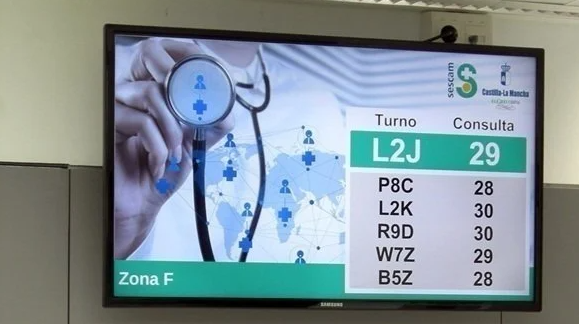
\includegraphics[width=0.8\textwidth]{hospital.png}
	\subcaption*{\textit{Nota.} \citeauthor{pantallasChange}}
    \end{subfigure}
	\label{fig:hospital}
\end{figure}
\vspace{-1.0\baselineskip}
Ahora bien, la implementación de pantallas para poder mostrar información en hospitales no siempre a generado resultados positivos. En los casos en que no fueron acompañadas por avisos sonoros, aquellos que sufran impedimentos visuales ya no pudieron saber cosas como dónde debían pasar a consultar ni a que sala les correspondía entrar. Las soluciones en ocasiones fueron pedir ayuda a auxiliares, atención del paciente u otros, quitando así la posibilidad de ser independientes a estos pacientes \parencite{pantallasChange}.

La utilización de pantallas no se limita a los hospitales únicamente, sino que otros sectores las han implementado para mostrar determinada información. Por ejemplo, en algunos locales de comida rápida pueden verse pantallas en la zona donde se retiran los pedidos que indican a quienes están esperando que ya se está realizando o que ya se puede retirar su orden. Para esto último pueden usar un número indicado en el tique de compra y otro para el puesto, lo cual es similar al caso de los hospitales en que se indica la sala a la cual pasar y el número asignado al turno.

De hecho, incluso en algunos colectivos pueden verse pantallas que muestran contenido recreacional para volver más ameno el viaje o que incluso permiten ver información relevante sobre el viaje. Por ejemplo, se instaló hace años pantallas LED en algunos colectivos que ofrecen información sobre los recorridos de las líneas (fig.~\ref{fig:colectivo}) y anuncian las paradas más importantes \parencite{lacapitalColectivos}.
\begin{figure}[H]
	\caption{Preguntados}
    \begin{subfigure}{1.0\textwidth}
	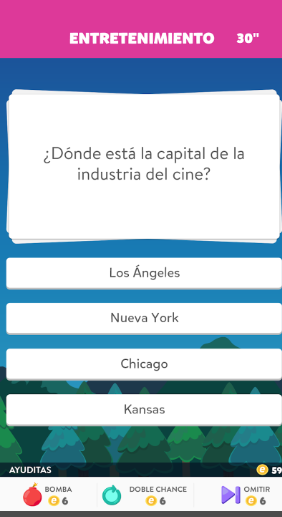
\includegraphics[width=0.4\textwidth]{preguntados.png}
	\subcaption*{\textit{Nota.} \citeauthor{playStorePreguntados}}
    \end{subfigure}
	\label{fig:preguntados}
\end{figure}
\vspace{-1.0\baselineskip}
Dado que se busca usar una trivia para el proyecto en cuestión, se buscó información de un videojuego basado en dicho formato. El videojuego para celulares Preguntados es una trivia usada por millones de personas en el mundo, en especial en Latinoamérica, que permite competir contra amigos. Se contesta entre cuatro posibles respuestas sobre una temática dada (fig.~\ref{fig:preguntados}). Contiene algunas ayudas, como por ejemplo una bomba para eliminar dos respuestas erroneas y también una opción para cambiar de pregunta. \parencite{minutouno}. Contiene preguntas que pertenecen a categorías como Entretenimiento, Deportes, Arte, Historia, Literatura, Geografía, Ciencia y Tecnología \parencite{abcPreguntados}.
\begin{figure}[H]
	\caption{Colectivo con pantalla que muestra información relevante}
    \begin{subfigure}{1.0\textwidth}
	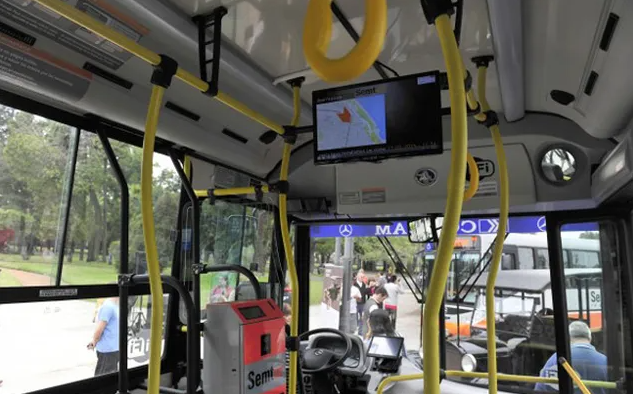
\includegraphics[width=0.8\textwidth]{colectivo.png}
	\subcaption*{\textit{Nota.} \citeauthor{lacapitalColectivos}}
    \end{subfigure}
	\label{fig:colectivo}
\end{figure}
\vspace{-1.0\baselineskip}
Los ejemplos de sistemas vigentes actualmente muestran algunas formas en que se resolvieron problemáticas similares a las que se debió enfrentar el proyecto actual. Elementos como la trivia y las indicaciones para distribuir pacientes son necesarios para resolverlas, y también la provisión de una salida sonora para el sistema demostró ser necesaria para así volver dar más accesibilidad al sistema.
\newpage
\section{Definición del problema}
Antes de desarrollar el sistema planteado, existían múltiples problemas en el sector de espera para internación del Hospital de Clínicas.

En primer lugar, los pacientes no sabían a ciencia cierta cuándo un puesto se encontraba libre, y al no existir un sistema informático que se los indicara, era necesario que se avise en voz alta. Esto no resultaba eficiente ni conveniente, por lo que quedaba clara la necesidad de implementar un sistema que, mediante una pantalla y una salida de audio, indique a los pacientes cuando puedan pasar a algún puesto.

Además, al tratarse de una espera para internación, la situación no resultaba amena para los pacientes, por lo que proveer un medio para amenizar el momento mediante la pantalla mencionada anteriormente podía resultar conveniente.

Por último, al contar con un edificio de grandes proporciones, no es fácil saber específicamente ciertas cosas como, por ejemplo, la ubicación de los distintos sectores de atención. Podía aumentarse el conocimiento de aspectos importantes como este mediante el uso de la pantalla para dar información que beneficie a los pacientes adicional a la de los puestos libres.

De esta forma, con una pantalla, un sistema de audio y una computadora podían atenderse los tres problemas utilizando un sistema que indique los puestos libres, información sobre temas relevantes y una trivia referida a esos temas para volver más amena la espera.
\newpage
\section{Solución propuesta}
Para dar una solución a los problemas vistos, se necesitó contar con una lista de puestos libres que sólo muestre aquellos a los cuales los pacientes puedan pasar. En caso de que todos se encuentren libres, en su lugar se optó por mostrar un único mensaje que lo indique. Si ninguno se encuentra libre se muestra también un único mensaje para indicarlo. Cuando un puesto se libera, esto se indica también mediante la salida de audio.

Para mostrar la trivia se eligió usar una parte de la pantalla, en la que se muestre primero un texto con información relevante, luego un enunciado con unas posibles respuestas, y un timer. Una vez terminado el tiempo, se indica la respuesta correcta y un texto que brinda información relevante.
\newpage
\subsection{Determinación de metodologías y tecnologías a utilizar}
A la hora de determinar las metodologías y tecnologías que se usarán en el desarrollo del sistema, se debieron tener en cuenta ciertos factores que permitieran distinguir las mejores opciones de entre las demás. Para ello se prestó atención a los factores enumerados a continuación:

Para elegir metodologías:
\begin{itemize}
    \item Mejoramiento de la calidad
    \item Tiempo necesario para el desarrollo
    \item Aplicabilidad
    \item Capacidad de adaptación a cambios de requerimientos
\end{itemize}
Para elegir tecnologías:
\begin{itemize}
    \item Sencillez de uso
    \item Grado de adopción
    \item Rendimiento
    \item Mantenibilidad
    \item Dificultad de aprendizaje
    \item Aplicabilidad
\end{itemize}
Para determinar qué metodologías y tecnologías se usarán, se seguirá un criterio que permita ver cuáles son las más ventajosas. Para ello se utilizará el de suma y ponderación cualitativas. \textcite{scriven} explica lo siguiente sobre este criterio: 
\blockquote[p. 166]{Utiliza símbolos como pesos, por ejemplo: E = esencial, * = extremadamente valioso, \# = muy valioso, + = valioso, | = marginalmente valioso y 
0 = sin valor. La evaluación se realiza en tres pasos: 

1. Construcción de la lista de atributos: Se establece una lista de atributos para los 
productos a evaluar. Luego se le otorga a cada uno de los atributos un peso de 
referencia máximo (en forma de símbolo). Se eliminan los atributos que obtienen el 
peso 0, pues se los considera irrelevantes. 

2. Calificación de los atributos de cada producto: Se les asigna a los atributos de cada 
producto un símbolo que no puede exceder el peso de referencia máximo 
 correspondiente. Por ejemplo, si el peso de un atributo es \#, se lo puede calificar como 
\#, +, | o 0, pero no *. Si un producto obtiene una calificación menor que E en algún 
atributo cuyo peso de referencia es E, el producto se elimina. Si todos los productos 
obtienen la misma calificación en algún atributo, el atributo se elimina. 

3. Construcción del ranking: Para cada producto, se cuenta cuántos símbolos de cada 
tipo obtuvo, y según esos totales se ordenan los productos. A veces hace falta 
comparar más detalladamente algún par de productos. Por ejemplo: 3*, 4\#, 2+ y 1| es 
sin duda mejor que 2*, 5\#, 2+ y 1|, pero no está claro, a priori, si es mejor que 2* y 8\#. }
\subsubsection{Metodologías}
Para realizar el desarrollo del proyecto se deberán elegir algunas metodologías a seguir que permitan asegurar la calidad del sistema, el cumplimiento de objetivos y el uso eficaz del tiempo. A continuación se explican algunas metodologías de entre las cuales se deberán elegir aquellas que se van a usar.
\begin{itemize}
    \item Kanban
    \item Test Driven Development
    \item Extreme Programming
    \item Desarrollo en cascada
\end{itemize}
El proceso Kanban consta de tres partes principales: el tablero, la lista y la tarjeta. El tablero contiene el flujo de trabajo, la lista contiene una serie de tarjetas, y la tarjeta es un producto que debe crearse o una tarea que debe realizarse. Las tareas se van trasladando a distintas listas conforme se vayan realizando. Las tarjetas pueden indicar en su reverso cosas como \textit{checklists} o su fecha límite para ser completadas. Se asignan prioridades a las tarjetas y se logra organizar el trabajo estableciendo cuáles son las cosas que deben hacerse con mayor urgencia \parencite{completeGuideAgile}.

Por otra parte, los usuarios de la metodología denominada Test Driven Development ponen el énfasis en confeccionar tests unitarios para cada parte del código antes de realizar su implementación. Esta metodología se compone de 3 pasos que se repiten constantemente: escribir un test que falle, realizar la implementación para que se apruebe dicho test, y por último refactorizar esa implementación \parencite[pp. 19-20]{testingJavascript}.

Extreme Programming (XP) es una metodología ágil enfocada en entregar el sistema que se necesita, cuando se lo necesita \parencite{xp}.

XP promueve que en un proyecto haya una retroalimentación, respeto, comunicación, simplicidad y coraje. La comunicación entre miembros de un equipo que usa esta metodología debe ser fluida, permitiendo que se pueda indicar incluso cuáles son aquellos aspectos del proyecto que pueden llegar a traer problemas a futuro. En lugar de planificar a detalle cada parte del sistema con mucha antelación, se prefiere tener una buena idea general del mismo y recién ahondar en los detalles de cada parte cuando sea el momento apropiado. Las implementación se caracteriza por ser simple, buscando pasar los tests confeccionados para asegurarse del buen funcionamiento del sistema. En lugar de entregar el proyecto sólo después de haber implementado todos los requerimientos del cliente, se le puede brindar acceso a una versión anterior, que implemente parte de dichos requerimientos y que permita empezar a usarla más rápido, gracias a haber sido desarrollada incrementalmente. Las funcionalidades principales son las elegidas para implementarse en los componentes iniciales del sistema, y los cambios realizados se integran de manera continua, almacenándose en el repositorio de proyecto incluso varias veces al día \parencite{agileProjectManagement}.

La metodología de desarrollo en cascada consta de distintas fases secuenciales, define de manera clara los procesos del proyecto y permite determinar de antemano los requerimientos para su realización. Es el método tradicional para hacer proyectos, caracterizado por su baja capacidad de adaptación al cambio en los requerimientos. Las fases que lo componen son la de requisitos, análisis, diseño, implementación, prueba, despliegue y mantenimiento \parencite{iepWaterfall}.

Entre las ventajas del desarrollo en cascada se encuentran que mantiene el trabajo organizado, define claramente los objetivos desde sus fases iniciales y permite identificar la fase en la cual se ha cometido algún error. Entre su desventajas están la obligatoriedad de terminar una fase para poder pasar a la siguiente, la demora en encontrar fallos y la dificultad para dividir en fases ordenadas el desarrollo de los proyectos de mayor tamaño \parencite{crehanaWaterfall}.

En cuanto a la aplicabilidad, la metodología XP es la única de entre las destacadas previamente que no puede utilizarse ya que requiere contar con un equipo compuesto por más de una persona para poder realizar la programación por pares, la cual ha sido descripta como una de las doce prácticas originales de XP \parencite{agileAlliance}.

Al asignar pesos como calificaciones a los atributos a evaluar, y luego hacer lo mismo a los atributos de cada metodología, se llegó a la distribución que se muestra en la fig.~\ref{fig:metodologias}.
\begin{figure}[H]
	\caption{Calificaciones para metodologías}
    \begin{subfigure}{1\textwidth}
	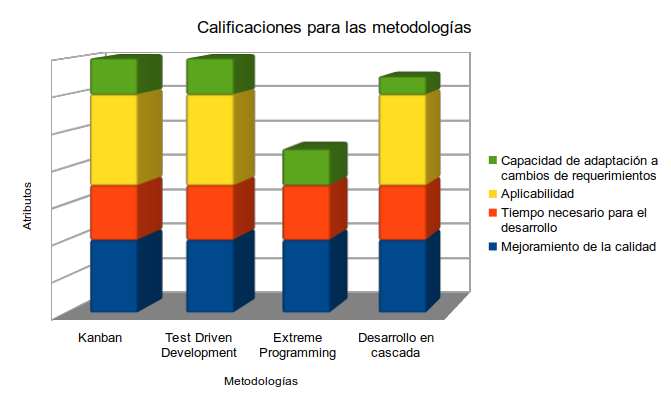
\includegraphics[width=1\textwidth]{calificaciones para metodologias.png}
    \end{subfigure}
	\label{fig:metodologias}
\end{figure}
\vspace{-1.0\baselineskip}
Como se detalla en el Anexo I, Kanban y Test Driven development fueron las metodologías elegidas para el desarrollo del sistema.
\subsubsection{Lenguaje de programación del lado del cliente}
Para el desarrollo del lado del cliente (frontend) se elegió entre los siguientes lenguajes de programación:
\begin{itemize}
    \item JavaScript
    \item TypeScript
\end{itemize}
Hablando sobre JavaScript, \textcite{mdnJs} detalla lo siguiente:
\blockquote{JavaScript (JS) es un lenguaje de programación ligero, interpretado, o compilado justo-a-tiempo (just-in-time) con funciones de primera clase. Si bien es más conocido como un lenguaje de scripting (secuencias de comandos) para páginas web, y es usado en muchos entornos fuera del navegador, tal como Node.js\textsuperscript{\textregistered}, Apache CouchDB y Adobe Acrobat. JavaScript es un lenguaje de programación basada en prototipos, multiparadigma, de un solo hilo, dinámico, con soporte para programación orientada a objetos, imperativa y declarativa (por ejemplo programación funcional).}
Por otra parte, el lenguaje TypeScript es un superconjunto de JavaScript, orientado a objetos y compilado \parencite{msTs}. Se diferencia de JavaScript en que permite especificar los tipos de datos que se pasan en el código, pudiendo reportar errores cuando los tipos de datos no coinciden en el momento de compilación \parencite{w3schoolsTs}. 

Por su sencillez de uso se lo considera un lenguaje fácil de aprender. En cuanto a su grado de adopción, JavaScript es el lenguaje de programación más popular del mundo \parencite{w3schoolsJs}. 

En cuanto al rendimiento de JavaScript, un uso incompetente del mismo lleva a un empeoramiento de la velocidad del sistema. Es un lenguaje que permite escribir código muy ineficiente. Sin embargo, cada vez los motores para este lenguaje están más optimizados, al punto de que en la actualidad se encuentra bien optimizado y ya no es necesario preocuparse por cada línea de código \parencite{arturWojnar}. Usar JavaScript puede enriquecer la experiencia, pero excederse en su uso afecta negativamente a la velocidad de un sitio web \parencite{timVanSchie}.

Al ser un superconjunto de JavaScript, el código, sea este eficiente o no, puede dar un rendimiento similar usando TypeScript, por lo que sus ventajas e inconvenientes son similares en este apartado.

Al hacer un boceto, podría comenzarse a partir de un lienzo en blanco o de una hoja con guías y reglas. Al hacer un proyecto en JavaScript, se parte desde dicho lienzo en blanco, mientras que en TypeScript el tipado estático brinda ayuda adicional, similar a las guías y reglas. TypeScript es una gran herramienta para crear código que sea mantenible \parencite{hao}. 

En cuanto a la dificultad de aprendizaje, si ya se cuenta con conocimientos de JavaScript, TypeScript no es muy difícil de aprender \parencite{freecodecampTs}. Si no se cuenta con los fundamentos de programación necesarios esto puede ser un desafío, mientras que en otros casos puede ser algo extremadamente sencillo \parencite{thecodebytes}. Ahora bien, sigue siendo más fácil de aprender JavaScript que TypeScript \parencite{isJsHardToLearn}.

Al asignar pesos como calificaciones a los atributos a evaluar, y luego hacer lo mismo a los atributos de cada metodología, se llegó a la distribución que se muestra en la fig.~\ref{fig:lenguajesFrontend}.
\begin{figure}[H]
	\caption{Calificaciones para lenguajes frontend}
    \begin{subfigure}{1\textwidth}
	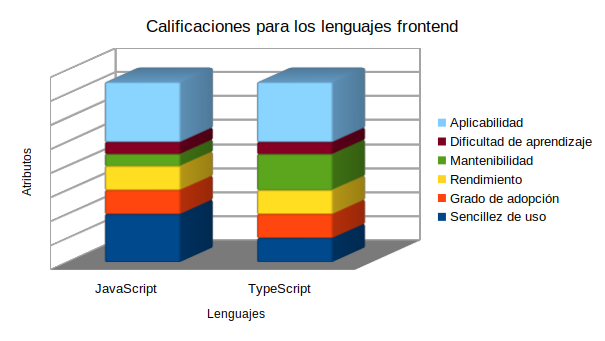
\includegraphics[width=1\textwidth]{calificaciones para lenguajes frontend.png}
    \end{subfigure}
	\label{fig:lenguajesFrontend}
\end{figure}
\vspace{-1.0\baselineskip}
Como se detalla en el Anexo I, luego de realizar el proceso de selección se determinó que JavaScript sería el lenguaje a usar para desarrollar el sistema.
\subsubsection{Framework para CSS}
En cuanto a los frameworks para CSS, se eligió entre las siguientes opciones:
\begin{itemize}
    \item Bootstrap
    \item Tailwind
\end{itemize}

Bootstrap permite crear sitios web rápidos y responsivos, contanddo con una caja de herramientas poderosa, extensible y con gran cantidad de características. Permite usar clases para personalizar la apariencia de componentes, por ejemplo modificando su posicionamiento, tamaño, colores y efectos \parencite{bootstrapOfficial}.

Tailwind permite crear sitios web modernos rápidamente sin dejar el HTML. Permiten crear diseños a través de clases directamente en el maquetado. Es de bajo nivel, dando acceso a personalizar los componentes al grado de lograr que incluso conservando la misma paleta de colores y escalado de tamaño, puedan tener una apariencia completamente diferente. Además es pequeño, lo que lleva a que el cliente solo deba descargar archivos de poco tamaño \parencite{tailwindOfficial}.

Bootstrap es fácil de aprender. Hay una gran cantidad de información en internet para verlo \parencite{hostingerBoostrap}. Su sencillez en el uso, excelente documentación y soporte de la comunidad también son algunos puntos a su favor, y ha llegado a ser el framework para CSS más usado \parencite{developerpitstop}. Ahora bien, el código puede ser difícil de mantener y estar desorganizado, lo cual es una clara desventaja \parencite{tenclouds}.

Tailwind permite crear diseños responsivos, y es sencillo de escribir y mantener código creado con este framework \parencite{hubspot}. También es fácil de aprender para quienes tengan un conocimiento previo de CSS \parencite{kinsta}. Aunque puede ser motivo de preocupación la mantenibilidad del código escrito en Tailwind, la realidad es que incluso leer líneas escritas en versiones antiguas puede ser simple y claro \parencite{oliverDavies}. 

Ahora bien, largas líneas de nombres descriptivos de clases de Tailwind pueden volverse difíciles de comprender, por lo que en producción pueden traer complicaciones para ser mantenidas \parencite{shiminZhang}. Este framework está enfocado en el rendimiento y busca usar el menor tamaño posible de archivos CSS generando solo aquel código que de verdad se usa en el proyecto \parencite{tailwindDocsOptimizing}.

Al asignar pesos como calificaciones a los atributos a evaluar, y luego hacer lo mismo a los atributos de cada metodología, se llegó a la distribución que se muestra en la fig.~\ref{fig:frameworksCSS}.
\begin{figure}[H]
	\caption{Calificaciones para frameworks para CSS}
    \begin{subfigure}{1\textwidth}
	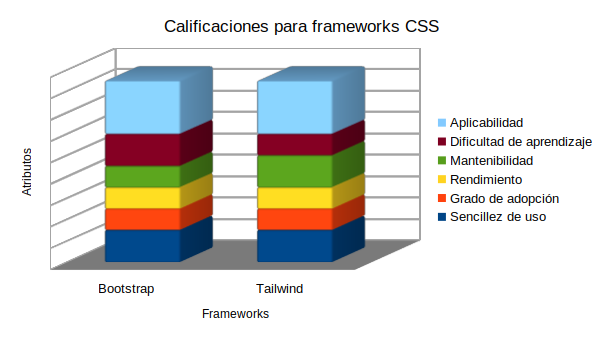
\includegraphics[width=1\textwidth]{calificaciones para frameworks css.png}
    \end{subfigure}
	\label{fig:frameworksCSS}
\end{figure}
\vspace{-1.0\baselineskip}
Como resultado del proceso de selección detallado en el Anexo I, se determinó que el framework Tailwind sería la opción elegida para el desarrollo del sistema.
\subsubsection{Framework o biblioteca frontend}
Para desarrollar el lado del cliente (frontend) del sistema también se debió elegir un framework o biblioteca. Las opciones que se consideraron fueron las siguientes:
\begin{itemize}
    \item Angular
    \item React
    \item Vue.js
\end{itemize}
 Angular es usado por millones de desarrolladores, cuenta con diversas herramientas y permite entregar aplicaciones web con confianza \parencite{angularHome}. Los proyectos que lo utilizan pueden ser eficientes y sofisticados, y se caracterizan por ser aplicaciones de una sola página. Provee injección de dependencias, para lo cual se utilizan los tipos de TypeScript \parencite{angularDocsIntroduction}. Además es fácil para aprender \parencite{w3schoolsAngular}. 

 React es una biblioteca que crear interfaces de usuario web y nativas, construyendolas a partir de componentes. Al utilizar React se puede usar código y marcado para crear los componentes, siendo estos funciones de JavaScript. Esto contribuye a que sean fáciles de crear, mantener y eliminar \parencite{reactOfficialHome}.

 Vue.js es un framework versátil para JavaScript con un buen rendimiento \parencite{vueOfficialHome}. Se usa para crear interfaces de usuario de manera práctica y rápida. Su curva de aprendizaje es la más sencilla comparado con las otras dos opciones. Puede empezar a usarse de manera progresiva, por ejemplo al migrar proyectos. Mientras React se centra más en un enfoque orientado a la programación en JavaScript, Vue.js está más enfocado en HTML y en los sistemas de plantillas \parencite{manz}.

Más de dos millones de sitios web están usando React. Los componentes en React son fáciles de depurar. Gracias a que usa el Virtual DOM, solo se actualizan los objetos que hayan cambiado, lo cual lleva a que el renderizado sea más veloz.  \parencite{galikReact}.

Diferentes encuestas muestran resultados de uso distintos de cada una de estas tecnologías. La encuesta de Stack Overflow que mide el uso de las tecnologías más relevantes (fig.~\ref{fig:stackOverflowSurvey}) pone en primer lugar a React, segundo a Angular y tercero a Vue.js; mientras que otra encuesta de Jet Brains enfocada en los frameworks web (fig.~\ref{fig:jetBrainsSurvey}) ubica a React en el primer puesto, Vue.js en el segundo y Angular en el cuarto. El uso de Vue.js en particular puede verse, por ejemplo, en grandes compañías como Adobe y Netflix \parencite{scalablepathVue}. En cuanto a la cantidad de estrellas en GitHub, Vue.js está en primer lugar, seguido por React y luego por Angular \parencite{codeinwp}.

\begin{figure}[H]
	\caption{Uso de las principales tecnologías desde 2016 hasta 2021}
    \begin{subfigure}{1.0\textwidth}
	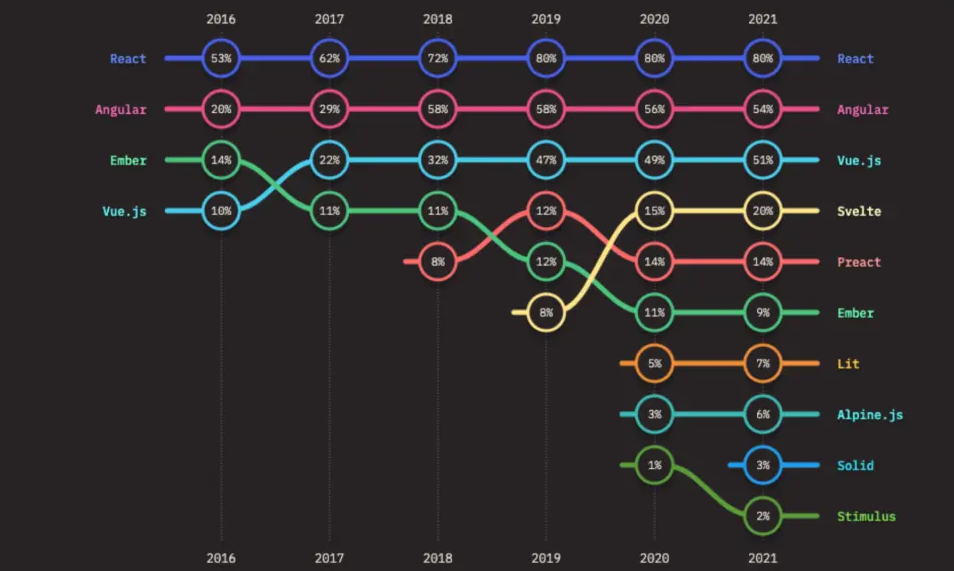
\includegraphics[width=0.8\textwidth]{vue-usage-from-2016-to-2021.png}
	\subcaption*{\textit{Nota.} 2022 Stack Overflow Survey.}
    \end{subfigure}
	\label{fig:stackOverflowSurvey}
\end{figure}
\vspace{-1.0\baselineskip}

\begin{figure}[H]
	\caption{10 Frameworks Web más usados en 2021}
    \begin{subfigure}{1.0\textwidth}
	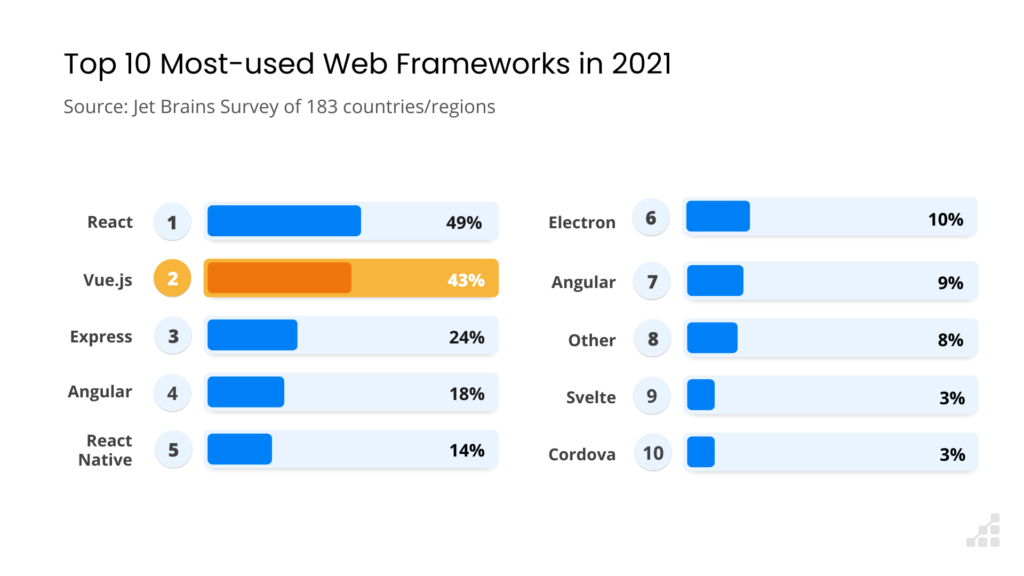
\includegraphics[width=0.9\textwidth]{most-used-web-frameworks-2021-survey-1-1024x576.png}
	\subcaption*{\textit{Nota.} Jet Brains Survey of 183 countries/regions 2021.}
    \end{subfigure}
	\label{fig:jetBrainsSurvey}
\end{figure}
\vspace{-2.0\baselineskip}

En Angular se usa una arquitectura basada en componentes que al ser fácilmente reemplazables permiten mantener el código de una manera más simple, y el basarse en TypeScript también contribuye a que esta tarea sea más amena. \parencite{altexsoftAngular}. Por otra parte, Vue.js cuenta con su Composition API que permite manejar el estado y la lógica en componentes de una forma flexible y modular, lo que mejora su mantenibilidad \parencite{theodosiou}.

Para quienes tienen conocimiento de JavaScript, React será más fácil y productivo, mientras que Vue resultará una mejor opción para principiantes \parencite{digitalya}. Vue.js es especialmente sencillo de usar para aplicaciones más pequeñas, pero cuando los proyectos se vuelven más complejos, depender únicamente de plantillas se torna cada vez más difícil, por lo que React resulta más fácil de usar para aplicaciones más grandes \parencite{stxnext}.

Al asignar pesos como calificaciones a los atributos a evaluar, y luego hacer lo mismo a los atributos de cada metodología, se llegó a la distribución que se muestra en la fig.~\ref{fig:frameworksFrontend}.
\begin{figure}[H]
	\caption{Calificaciones para frameworks frontend}
    \begin{subfigure}{1\textwidth}
	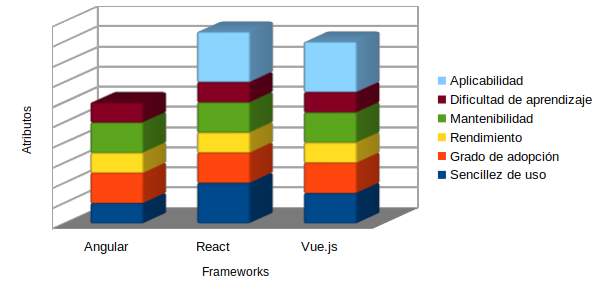
\includegraphics[width=1\textwidth]{calificaciones para frameworks frontend.png}
    \end{subfigure}
	\label{fig:frameworksFrontend}
\end{figure}
\vspace{-1.0\baselineskip}
Como resultado del proceso de selección detallado en el Anexo I, se determinó que React sería la opción elegida para el desarrollo del sistema.
\subsubsection{Lenguaje de programación y framework backend}
Para el desarrollo del lado del servidor (backend) se elegió entre los siguientes lenguajes de programación y frameworks:
\begin{itemize}
    \item Java y Spring
    \item Node.js\textsuperscript{\textregistered} y Express.js
\end{itemize}
Java es un lenguaje de programación y plataforma para computación, lanzado inicialmente por Sun Microsystems en 1995 \parencite{whatIsJava}. Algunas de sus características son su orientación a objetos, portabilidad, rendimiento soporte para concurrencia mediante el uso de múltiples hilos de ejecución \parencite{featuresJava}.

Spring es el framework para desarrollo de aplicaciones para Java empresarial más usado. El objetivo de quienes lo utilizan es obtener code fácilmente testeable, reusable y con un rendimiento elevado. Es modular y da soporte a la inyección de dependencias \parencite{tutorialspointSpring}.

Node.js\textsuperscript{\textregistered} es un entorno de ejecución de JavaScript orientado a eventos asíncronos que permite crear aplicaciones de red escalables. Contrasta con otros modelos de concurrencia basados en los hilos de Sistema Operativo los cuales suelen ser difíciles de usar y relativamente ineficientes, en su lugar usa un bucle de eventos \parencite{aboutNode}.

Express.js es un framework para Node.js\textsuperscript{\textregistered} diseñado para construir aplicaciones web y que se convirtió en el más usado para este entorno de ejecución. Es minimalista, rápido y muy fácil de usar \parencite{kinstaExpress}.

Java es fácil de aprender y depurar ya que fue diseñado para también ser fácil de usar \parencite{ibmJava}. Esto es así aún siendo un lenguaje más complejo que JavaScript \parencite{lighthouselabsJavaVSJavscript}. Datos de encuestas de Stack Overflow muestran java ya no es el lenguaje más usado aunque permanece entre los más populares, pasando de un 41,1\% de uso en 2019 a un 33,27\% en 2022 \parencite{devmJava}. En cuanto al rendimiento, Java es bastante rápido pero utiliza mucha memoria \parencite{akkiJava}.

Spring es muy usado para el desarrollo profesional con Java debido a su sencillez de uso, flexibilidad, documentación y soporte de la comunidad \parencite{flexipleJava}. Ahora bien, su curva de aprendizaje es empinada, por lo que resulta difícil para los desarrolladores relativamente inexpertos \parencite{adservio}. Al usar inyección de dependencias facilita el mantenimiento del código \parencite{turingSpring}.

Express.js permite manejar pedidos usando funciones modulares, pequeñas y mantenibles. Es fácil de aprender ya que utiliza JavaScript, lo que permite usarlo sin necesitar aprender otro lenguaje \parencite{linuxhintExpress}. 

Node.js\textsuperscript{\textregistered} es considerado el framework más usado por los desarrolladores en todo el mundo, según una encuesta del 2022 \parencite{statistaFrameworks}. El uso de funciones anónimas puede hacer que el código sea poco mantenible, por lo que es conveniente evitarlas y también estructurar las funciones callbacks \parencite{packtpub}. Incluso para un desarrollador Javascript Junior, Node.js\textsuperscript{\textregistered} se considera una tecnología que requiere menos esfuerzo y tiempo de aprendizaje \parencite{simplilearnNode}.

Al asignar pesos como calificaciones a los atributos a evaluar, y luego hacer lo mismo a los atributos de cada metodología, se llegó a la distribución que se muestra en la fig.~\ref{fig:lenguajesFrameworksBackend}.
\begin{figure}[H]
	\caption{Calificaciones para lenguajes y frameworks backend}
    \begin{subfigure}{1\textwidth}
	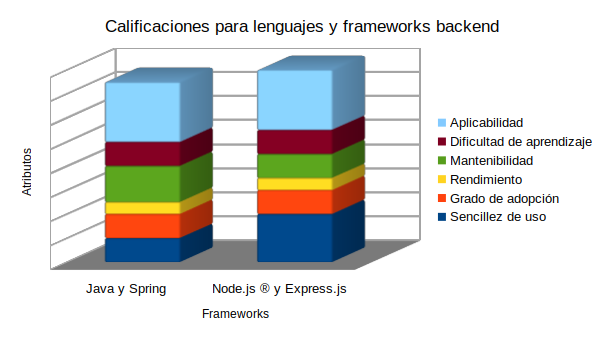
\includegraphics[width=1\textwidth]{calificaciones para lenguajes y frameworks backend.png}
    \end{subfigure}
	\label{fig:lenguajesFrameworksBackend}
\end{figure}
\vspace{-1.0\baselineskip}
Como resultado del proceso de selección detallado en el Anexo I, se determinó que Node.js\textsuperscript{\textregistered} junto con Express.js serían las opciones elegidas para el desarrollo del sistema.
\subsubsection{Base de datos}
Para el desarrollo de la base de datos se elegió entre los siguientes sistemas gestores:
\begin{itemize}
    \item MongoDB
    \item MySQL
    \item PostgreSQL
\end{itemize}
MongoDB es una base de datos basada en documentos escalable y flexible. Su modelo de documentos es simple de aprender y de usar, de hecho los datos se almacenan en documentos con un formato similar a JSON \parencite{whatIsMongoDBOfficial}. Es considerada la base de datos moderna más usada por el quinto año consecutivo \parencite{mongoOfficialHome}.

MySQL es el sistema gestor de base de datos de código abierto más popular. Utiliza el modelo relacional basado en tablas y utiliza archivos físicos optimizados para la velocidad. Para brindar acceso a las bases de datos se usa el lenguaje SQL. Este sistema es muy rápido y fácil de usar \parencite{whatIsMySQLOracle}.

PostgreSQL es un sistema gestor de base de datos objeto-relacional con un buen rendimiento y confiabilidad \parencite{postgreHome}. Intenta mantener conformidad con el estándar SQL sin que ello contradiga características tradicionales ni lleve a malas decisiones en cuanto a su arquitectura. De hecho contiene una gran cantidad de características que buscan ayudar a los desarrolladores a construir aplicaciones \parencite{postgreAbout}.

MongoDB puede manejar grandes cantidades de datos sin estructurar mucho más rápido que MySQL y PostgreSQL, pero tiene un alto consumo de memoria e incluso puede tener algún problema ocasional de velocidad en entornos en la nube \parencite{mongoMysqlComparison}. En este sistema cada documento se almacena en la base de datos junto a objetos de datos relacionados y encapsulados juntos, lo que permite extraer datos con una única operación. De esta forma MongoDB aumenta el rendimiento, la velocidad y la sencillez de mantenimiento \parencite{vsoftconsultingMongo}.

Se considera que MySQL es confiable y mantenible, lo que permite que los administradores de bases de datos no tengan que perder tiempo solucionando problemas de rendimiento y de tiempo de inactividad \parencite{dbquestMysql}. El lenguaje SQL, usado por MySQL y PostreSQL para acceder a las bases de datos, es fácil de aprender, pudiendo a prenderse en pocas semanas en caso de contar con conocimientos de programación previos \parencite{thinkfulSql}.

PostgreSQL tiene bajos costos operativos, es fácil de usar y de mantener \parencite{topcoderPostgresql}. Su cuota de mercado es de 17,32\%, mientras que la de MySQL es de 44,68\% \parencite{marketShareDb}.

Al asignar pesos como calificaciones a los atributos a evaluar, y luego hacer lo mismo a los atributos de cada metodología, se llegó a la distribución que se muestra en la fig.~\ref{fig:dbms}.
\begin{figure}[H]
	\caption{Calificaciones para Sistemas Gestores de Base de Datos}
    \begin{subfigure}{1\textwidth}
	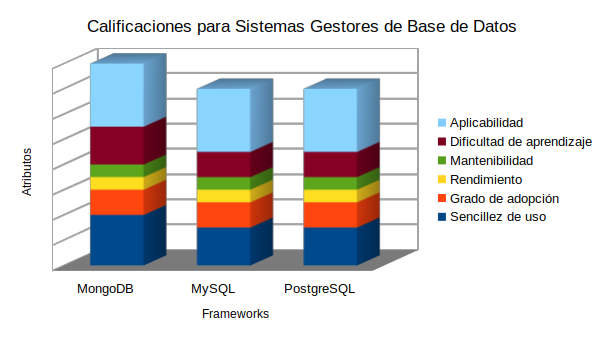
\includegraphics[width=1\textwidth]{calificaciones para dbms.png}
    \end{subfigure}
	\label{fig:dbms}
\end{figure}
\vspace{-1.0\baselineskip}
Como resultado del proceso de selección detallado en el Anexo I, se determinó que MongoDB sería la opción elegida para el desarrollo del sistema.
\subsubsection{Testing}
Para el testing del proyecto se elegió entre los siguientes frameworks:
\begin{itemize}
    \item Jasmine
    \item Jest
    \item JUnit
    \item Mocha
\end{itemize}
Jasmine es un veloz framework para desarrollo guiado por comportamiento que permite realizar testing de código escrito en JavaScript. Puede usarse para realizar los tests tanto para el navegador como para Node.js \textsuperscript{\textregistered}. Tiene una sintaxis sencilla para poder escribir fácilmente los tests \parencite{jasmineOfficialHome}. En este framework se escriben specs, que contienen expectativas que prueban el estado del código \parencite{jasmineYourFirstSuite}. Solo ejecuta las specs en paralelo cuando se cuenta con por lo menos la versión 5.0 del paquete de NPM Jasmine y se pasa el argumento de línea de comandos correspondiente \parencite{jasmineFrequentlyAskedQuestions}. 

En cuanto a Jest, este framework está centrado en la simplicidad y tiene un alto rendimiento gracias a que los tests se ejecutan de forma paralela. Es usado por muchas personas, llegando a encontrarse en más de 3 millones de repositorios públicos de GitHub \parencite{jestOfficial}.

JUnit es un framework de testing unitario para Java. Es simple, por lo que toma menos tiempo \parencite{tutorialsPointJUnit}. Provee a los desarrolladores anotaciones, assertions y test runners para poder crear y correr las pruebas unitarias y así contribuir a mejorar la calidad del código \parencite{simplilearnJUnit}. Los tests en JUnit son ejecutados rápidamente, lo que permite correr una gran suite de pruebas en un corto período de tiempo \parencite{codeIntelligenceJUnit}.

Mocha es un framework de testing para JavaScript repleto de características que corre tanto en Node.js\textsuperscript{\textregistered} como en el navegador, haciendo que el testing asíncrono sea simple. Los tests corren de manera serializada, lo que lleva a que los reportes sean precisos, relacionando las excepciones sin capturar con los casos de testeo correctos \parencite{mochaHome}. Tiene una sintaxis simple y es veloz \parencite{mindkTesting}.

En cuanto a la aplicabilidad, Jest, Mocha y Jasmine pueden ser usados para testear el código escrito en JavaScript, mientras que JUnit está destinado a testear el código escrito en Java. Esto implica que en el lado del cliente podían ser usados cualquiera de los tres primeros, mientras que en el backend se debería elegir entre ellos o JUnit dependiendo del lenguaje de programación seleccionado previamente.

En cuanto al grado de adopción, \textcite{stateofjsTesting} indican que 68\% de los encuestados usaron Jest, 53\% Mocha y 42\% Jasmine durante 2020. Por otra parte, JUnit es uno de los frameworks de testing para Java mas populares \parencite{headspinJUnit}.

Al asignar pesos como calificaciones a los atributos a evaluar, y luego hacer lo mismo a los atributos de cada metodología, se llegó a la distribución que se muestra en la fig.~\ref{fig:testing}.
\begin{figure}[H]
	\caption{Calificaciones para frameworks para testing}
    \begin{subfigure}{1\textwidth}
	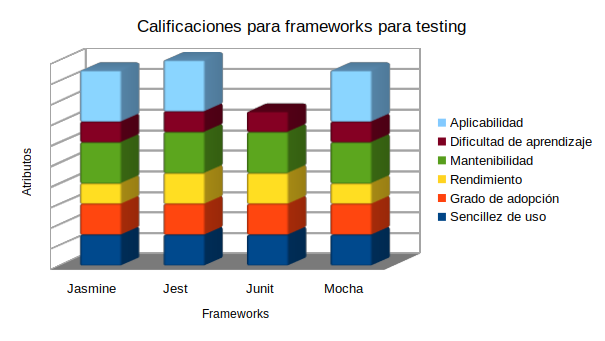
\includegraphics[width=1\textwidth]{calificaciones para frameworks para testing.png}
    \end{subfigure}
	\label{fig:testing}
\end{figure}
\vspace{-1.0\baselineskip}
Como resultado del proceso de selección detallado en el Anexo I, se determinó que Jest sería la opción elegida para el desarrollo del sistema.
\newpage
\subsection{Análisis de requisitos}
El sistema consta de dos requisitos principales: en primer lugar, aportar información sobre qué puestos se encuentran libres, actualizandose de manera automática y permitiendo a quienes lo controlen modificar dicha información; y en segundo lugar, brindar un método de recreación a través de una trivia, la cual también deberá ser editable por quienes controlen el sistema.

Por lo tanto, resulta necesario contar con la forma de efectuar altas, bajas, modificaciones y consultas para los registros de ambas partes del sistema, las cuales funcionarán gracias a la interacción entre el cliente web, el servidor y la base de datos, la cual almacenará información tanto de los puestos como de la triva.

A continuación se detallarán con mayor detalle los requisitos de la sección de trivia y de la correspondiente para los puestos libres y sus editores.
\subsubsection{Puestos}
Para que quienes estén esperando para ir a un puesto necesitan una forma para saber si hay puestos libres y cuáles son. Para ello en la pantalla principal se requiere mostrar los nombres de los puestos libres, y dar esa información también a través de una salida de audio.

Esta información debe actualizarse automáticamente y reflejar los datos ingresados por quienes controlen el sistema, que en principio deberían ser los empleados que ocupen los puestos, además de su jefe o encargado del sistema. Esos datos deben poder ingresarse con una interfaz de usuario que permita ocupar o liberar puestos de una manera sencilla y rápida, minimizando la curva de aprendizaje. 

Además, en caso de querer agregar o quitar puestos, o simplemente contar con un editor más elaborado, una interfaz alternativa, más avanzada es necesaria. De esta forma al usar por primera vez el sistema se podrán agregar los puestos y editar su información desde el editor de puestos avanzado, y una vez configurado los empleados podrán usar el editor simple para indicar cuando sus puestos se libern u ocupen.

Los datos deberán guardarse en una base de datos de tal forma que los mismos queden almacenados de forma persistente. En caso de apagarse la computadora en la cual corra la  base de datos, los mismos no se perderán, contrario a lo que ocurriría en caso de almacenarse en la memoria RAM.
\subsubsection{Trivia}
La trivia constará de preguntas con varias respuestas posibles, algunas correctas y otras incorrectas, y una explicación de por qué son correctas las respuestas así indicadas. Contar con animaciones para las transiciones entre preguntas y respuestas resulta apropiado para dar una mejor experiencia al usuario. Las trivias se podrán ver desde la pantalla principal junto con los puestos.

Cada trivia podrá ser ingresada por los encargados del sistema. Deberá proveerse una interfaz de usuario que permita también eliminar trivias y editarlas, modificando campos como la pregunta, las respuestas, cuáles son correctas y la explicación.
\newpage
\subsection{Especificaciones del sistema}
Para la base de datos se optó por usar MongoDB. Esto implicó que la conexión entre el servidor y la base de datos se realice a través de Mongoose. Este servidor se implementó con tecnologías basadas en JavaScript, como NodeJS\textsuperscript{\textregistered} y Express.js. El testing se realizó usando Jest. Para permitir el despliegue usando contenedores se usó Docker junto con Kubernetes.

Para el frontend se eligió crear un cliente web que fuera accesible desde un navegador de internet. Al igual que en el backend se usaron tecnologías basadas en JavaScript, en este caso React junto con Fluent UI, Tailwind y Vite.
\newpage
\subsection{Análisis del sistema}
La información necesaria para ambas partes del sistema se representó a través de documentos en la base de datos no relacional hecha con MongoDB. Estos documentos podían contar con dos estructuras, dependiendo si se trataba de trivias o de puestos.

Para los puestos, se usaron el nombre (cadena de caracteres) y su disponibilidad (booleano) como campos.

Para las trivias, se usaron la pregunta (cadena de caracteres), la explicación (cadena de caracteres) y las respuestas (vector de cadena de caracteres) como campos.

Por otra parte, un router fue usado para que al ingresar pedidos HTTP a determinadas URLs, el controlador apropiado lo procese. Un controlador para los pedidos relacionados con las trivias y otro para los puestos fueron usados. A su vez cada uno constó de funciones asíncronas que permitían, según su caso, gestionar pedidos de altas, bajas, modificaciones y consultas.

Mediante Jest se realizaron tests para verificar el buen funcionamiento del sistema, los mismos abarcan los pedidos tanto para trivias como para puestos de altas, bajas, modificaciones y consultas.

En cuanto al frontend, su principal componente incluye tanto una sección para ver las trivias de manera secuencial como otra para indicar los puestos que se encuentren libres. Para actualizar los puestos de forma automática se recurrió a la técnica de polling a través de Tanstack Query, el cual en intervalos recurrentes hace que el cliente pida datos nuevos al servidor para poder contar con información relevante sin necesidad de recargar la página manualmente.

El editor simple para puestos permite elegir a través de una lista desplegable el puesto a modificar y con un botón pasar su estado de libre a ocupado.

El editor avanzado para puestos permite agregar, quitar y editar puestos. Los datos que permite modificar son los nombres y las disponibilidades de cada puesto.

El editor de trivias permite agregar, quitar y editar trivias. En cada trivia pueden modificarse la pregunta, la explicación, las respuestas y la validez de cada una.
\newpage
\section{Resultados}
El sistema implementado consta de los componentes descriptos anteriormente, por lo que en esta sección podrán verse el aspecto que tomaron, detalles sobre su funcionalidad y características finales.

En la pantalla principal (fig.~\ref{fig:pantallaPrincipal}), ideada para usarse en una pantalla que sea vista por quienes estén esperando para pasar a un puesto libre, muestra aquellos puestos que estén libres y la sección de la trivia.
\begin{figure}[H]
	\caption{Pantalla principal del sistema}
    \begin{subfigure}{1\textwidth}
	\includegraphics[width=1\textwidth]{sirhc pantalla principal.png}
    \end{subfigure}
	\label{fig:pantallaPrincipal}
\end{figure}
\vspace{-1.0\baselineskip}
En el editor de puesto (fig.~\ref{fig:editorPuesto}), pensado para que cada empleado encargado de un puesto, permite que se elija un puesto y se indique su liberación u ocupación, lo cual se ve reflejado en la pantalla principal que se actualiza automáticamente.
\begin{figure}[H]
	\caption{Editor de puesto}
    \begin{subfigure}{1\textwidth}
	\includegraphics[width=1\textwidth]{sirhc editor de puesto.png}
    \end{subfigure}
	\label{fig:editorPuesto}
\end{figure}
\vspace{-1.0\baselineskip}
En el editor de puestos avanzado (fig.~\ref{fig:editorPuestosAvanzado}), necesario para un administrador del sistema, permite no solo liberar y ocupar puestos sino también cambiar sus nombres, agregar e incluso remover puestos.
\begin{figure}[H]
	\caption{Editor de puestos avanzado}
    \begin{subfigure}{1\textwidth}
	\includegraphics[width=1\textwidth]{sirhc editor de puestos avanzado.png}
    \end{subfigure}
	\label{fig:editorPuestosAvanzado}
\end{figure}
\vspace{-1.0\baselineskip}
En el editor de trivias (fig.~\ref{fig:editorTrivias}), necesario para un administrador del sistema, se pueden agregar, eliminar y editar trivias. Entre los campos que pueden editarse se encuentran las preguntas, respuestas y explicaciones de las trivias.
\begin{figure}[H]
	\caption{Editor de trivias}
    \begin{subfigure}{1\textwidth}
	\includegraphics[width=1\textwidth]{sirhc editor de trivias.png}
    \end{subfigure}
	\label{fig:editorTrivias}
\end{figure}
\vspace{-1.0\baselineskip}
Se incluyó un fondo de pantalla para las interfaz de usuario para que la misma tuviera un mejor aspecto visual, el mismo en primera instancia se intentó que estuviera relacionado con la medicina o incluso el mismo Hospital de Clínicas, sin embargo al dar un aspecto poco conveniente se optó por un fondo que, aunque pudiera parecer fuera de lugar (lo mismo podría decirse de la trivia, que es en realidad una funcionalidad fundamental del sistema), brinda un aspecto más ameno a una interfaz que, de otra forma, podría verse desagradable.

Al incluirse en el repositorio ubicado en: \href{https://github.com/charrassebastian/sirhc}{https://github.com/charrassebastian/sirhc} se encuentra tanto el código como también archivos de configuración para realizar el despliegue con Docker y Kubernetes.

Al usar contenedores se pueden aislar las capas del sistema (cliente, servidor y base de datos). Para contar con una versión disponible como parte de un portfolio de proyectos, en un servidor presente en una red local se realizó un despliegue aprovechando las tecnologías Docker y Kubernetes, y que al momento de redactar este informe puede accederse a través del siguiente enlace: \href{https://sirhc.sebastiancharras.tech}{https://sirhc.sebastiancharras.tech}.

Los tests implementados para la API permiten contar con un mayor grado de confianza en el sistema, asegurando el buen funcionamiento de esta parte esencial del backend, necesaria para que pueda usarse sin problemas. El testing no incluyó, por ejemplo, a los componentes del cliente, sino que se centró exclusivamente en la API, particularmente en el servidor.

La base de datos usa MongoDB, para lo que puede aprovecharse la imagen oficial de dicho software para crear un contenedor y correrlo de manera sencilla. Las versiones más recientes requieren soporte de instrucciones AVX en el procesador, por lo que en computadoras más antiguas y de gamas más bajas es posible encontrar incompatibilidades debido a este requisito. Sin embargo, usando una versión antigua es posible resolver este problema, como por ejemplo la versión 4.
\newpage
\section{Conclusiones}
La experiencia de desarrollo fue enriquecedora, contribuyendo a adquirir y reforzar conocimientos en diversas áreas del desarrollo, tanto sobre tecnologías como de metodologías.

Una de las cosas más importantes fue lo aprendido sobre la metodología Test Driven Development. Esta pone su foco en crear tests unitarios para cada código escrito, incluso escribiendo los tests antes que las implementaciones. De esta forma se asegura la calidad del producto, previniendo la entrega de productos defectuosos.

Ahora bien, aunque sea muchas veces vista de una manera muy positiva debido a las razones ya mencionadas, esta metodología de desarrollo puede llevar a que se tome más tiempo en crear un programa que realizando un uso menos frecuente de tests. Durante el desarrollo de este sistema, utilizar esta metodología en frontend demostró ser particularmente complejo en comparación con su uso en el backend, lo que llevó a que se decidiera enfocar la escritura de tests en asegurar el buen funcionamiento de la API, dejando de lado, entre otras cosas, el testeo de los componentes del frontend.

Por otra parte, las tecnologías usadas contribuyeron a la creación del sistema sin requerir cantidades de tiempo de aprendizaje demasiado grandes. Su sencillez de uso y amplia documentación, así como la extensa cantidad de bibliotecas disponibles hicieron que la implementación del sistema se realizara de una manera rápida.

Aunque la cantidad de tecnologías y de metodologías en las que se tuvo que ahondar para realizar el desarrollo fue mayor que en otros proyectos realizados, las elecciones tomadas hicieron que esto no llevara a un atraso en los tiempos de desarrollo ni a una merma en las características implementadas. Los nuevos conocimientos adquiridos y la experiencia con la metodología Test Driven Development son algunas de las cosas más útiles que se obtuvieron en este proyecto.
\newpage
\section{Referencias}
\begin{sloppypar}
\printbibliography[heading=none,category=cited]
\end{sloppypar}
\newpage
\section{Bibliografía}
\printbibliography[heading=none,notcategory=cited]
\newpage
\section{Anexos}
\subsection{Selección de metodologías y tecnologías}
\subsubsection{Selección de metodologías}
Para realizar la selección se usaron los mismos símbolos como pesos indicados en el ejemplo. Los pesos de referencia de los atributos para este caso son los siguientes:
\begin{itemize}
    \item Mejoramiento de la calidad - *
    \item Tiempo necesario para el desarrollo - \#
    \item Aplicabilidad - E
    \item Capacidad de adaptación a cambios de requerimientos - +
\end{itemize}
A continuación se indican los símbolos asignados a cada metodología como calificación por atributo.

Kanban
\begin{itemize}
    \item Mejoramiento de la calidad - *
    \item Tiempo necesario para el desarrollo - \#
    \item Aplicabilidad - E
    \item Capacidad de adaptación a cambios de requerimientos - +
\end{itemize}
Test Driven Development
\begin{itemize}
    \item Mejoramiento de la calidad - *
    \item Tiempo necesario para el desarrollo - \#
    \item Aplicabilidad - E
    \item Capacidad de adaptación a cambios de requerimientos - +
\end{itemize}
Extreme Programming
\begin{itemize}
    \item Mejoramiento de la calidad - *
    \item Tiempo necesario para el desarrollo - \#
    \item Aplicabilidad - 0
    \item Capacidad de adaptación a cambios de requerimientos - +
\end{itemize}
Desarrollo en cascada
\begin{itemize}
    \item Mejoramiento de la calidad - +
    \item Tiempo necesario para el desarrollo - \#
    \item Aplicabilidad - E
    \item Capacidad de adaptación a cambios de requerimientos - |
\end{itemize}
Al realizar este paso puede comprobarse que Extreme Programming no cumplió el requisito de aplicabilidad, por lo que no podría ser usada. Además, las metodologías restantes obtuvieron resultados idénticos para el campo de tiempo necesario para el desarrollo, por lo que dicho atributo debería ser eliminado. Esto da lugar a los siguientes resultados:

Kanban
\begin{itemize}
    \item Mejoramiento de la calidad - *
    \item Aplicabilidad - E
    \item Capacidad de adaptación a cambios de requerimientos - +
\end{itemize}
Test Driven Development
\begin{itemize}
    \item Mejoramiento de la calidad - *
    \item Aplicabilidad - E
    \item Capacidad de adaptación a cambios de requerimientos - +
\end{itemize}
Desarrollo en cascada
\begin{itemize}
    \item Mejoramiento de la calidad - +
    \item Aplicabilidad - E
    \item Capacidad de adaptación a cambios de requerimientos - |
\end{itemize}
Al elaborar el ranking, los resultados fueron los siguientes:
\begin{itemize}
    \item Kanban - 1E, 1* y 1+
    \item Test Driven Development - 1E, 1* y 1
    \item Desarrollo en cascada - 1E, 1+ y 1|
\end{itemize}
Por la escaza capacidad de adaptación a cambios de requerimientos del desarrollo en cascada, quedó en evidencia la necesidad de excluirla a la hora de desarrollar el sistema. Kanban y Test Driven development resultaron ser según el criterio aplicado las metodologías más apropiadas, por lo que se elegio usar ambas en el desarrollo del sistema.
\subsubsection{Selección de lenguajes frontend}
Al momento de seleccionar entre ambos lenguajes se optó por otorgar los siguientes pesos a los atributos a considerar:
\begin{itemize}
    \item Sencillez de uso - *
    \item Grado de adopción - +
    \item Rendimiento - +
    \item Mantenibilidad - \#
    \item Dificultad de aprendizaje - |
    \item Aplicabilidad - E
\end{itemize}
Al calificar mediante símbolos los atributos en cuestión de JavaScript y TypeScript, los resultados fueron los siguientes:

JavaScript
\begin{itemize}
    \item Sencillez de uso - *
    \item Grado de adopción - +
    \item Rendimiento - +
    \item Mantenibilidad - |
    \item Dificultad de aprendizaje - |
    \item Aplicabilidad - E
\end{itemize}
TypeScript
\begin{itemize}
    \item Sencillez de uso - +
    \item Grado de adopción - +
    \item Rendimiento - +
    \item Mantenibilidad - \#
    \item Dificultad de aprendizaje - |
    \item Aplicabilidad - E
\end{itemize}
Pueden observarse resultados idénticos entre ambas tecnologías para los campos de grado de adopción, rendimiento, dificultad de aprendizaje y aplicabilidad, por lo que se deben eliminar dichos atributos, dando lugar a los siguientes resultados:

JavaScript
\begin{itemize}
    \item Sencillez de uso - *
    \item Mantenibilidad - |
\end{itemize}
TypeScript
\begin{itemize}
    \item Sencillez de uso - +
    \item Mantenibilidad - \#
\end{itemize}
El ranking quedó de la siguiente forma:
\begin{itemize}
    \item JavaScript - 1* y 1|
    \item TypeScript - 1\# y 1+
\end{itemize}
La ventaja de TypeScript en cuanto a mantenibilidad por sobre JavaScript permitió compensar su menor sencillez de uso, por lo que entregó un resultado más equilibrado. La importancia otorgada a la sencillez de uso era mayor que la dada a la mantenibilidad, por lo que si bien ambas opciones eran buenas candidatas para el  desarrollo en cuestión, se optó por usar JavaScript.
\subsubsection{Selección de framework para CSS}
Al momento de optar por una de las dos opciones, a los atributos a considerar se les asignaron los siguientes símbolos como pesos:
\begin{itemize}
    \item Sencillez de uso - \#
    \item Grado de adopción - +
    \item Rendimiento - +
    \item Mantenibilidad - *
    \item Dificultad de aprendizaje - \#
    \item Aplicabilidad - E
\end{itemize}
Los frameworks en cuestión recibieron estas calificaciones para cada atributo:

Bootstrap
\begin{itemize}
    \item Sencillez de uso - \#
    \item Grado de adopción - +
    \item Rendimiento - +
    \item Mantenibilidad - +
    \item Dificultad de aprendizaje - \#
    \item Aplicabilidad - E
\end{itemize}
Tailwind
\begin{itemize}
    \item Sencillez de uso - \#
    \item Grado de adopción - +
    \item Rendimiento - +
    \item Mantenibilidad - \#
    \item Dificultad de aprendizaje - +
    \item Aplicabilidad - E
\end{itemize}
Los atributos sencillez de uso, grado de adopción, rendimiento y aplicabilidad recibieron pesos idénticos para ambas tecnologías, por lo que debieron eliminarse, dando lugar a los siguientes resultados:

Bootstrap
\begin{itemize}
    \item Mantenibilidad - +
    \item Dificultad de aprendizaje - \#
\end{itemize}
Tailwind
\begin{itemize}
    \item Mantenibilidad - \#
    \item Dificultad de aprendizaje - +
\end{itemize}
Lo que lleva a que se forme el siguiente ranking:
\begin{itemize}
    \item Tailwind - 1\# y 1+
    \item Bootstrap - 1\# y 1+
\end{itemize}
Aunque los resultados lucen idénticos, Tailwind recibió una calificación superior en el campo de mantenibilidad, mientras que Bootstrap la recibió para el de dificultad de aprendizaje, que era menos valorado. Esto llevó a que se optara por usar tailwind ya que era más importante contar con un código mantenible que con un framework de CSS más sencillo de aprender.
\subsubsection{Selección de frameworks o bibliotecas frontend}
Para elegir entre las opciones detalladas anteriormente, se otorgaron los siguientes pesos a los atributos a tener en cuenta:
\begin{itemize}
    \item Sencillez de uso - *
    \item Grado de adopción - \#
    \item Rendimiento - +
    \item Mantenibilidad - \#
    \item Dificultad de aprendizaje - +
    \item Aplicabilidad - E
\end{itemize}
Luego se asignó pesos por cada atributo a las tecnologías en cuestión:

Angular
\begin{itemize}
    \item Sencillez de uso - +
    \item Grado de adopción - \#
    \item Rendimiento - +
    \item Mantenibilidad - \#
    \item Dificultad de aprendizaje - +
    \item Aplicabilidad - 0
\end{itemize}
React
\begin{itemize}
    \item Sencillez de uso - *
    \item Grado de adopción - \#
    \item Rendimiento - +
    \item Mantenibilidad - \#
    \item Dificultad de aprendizaje - +
    \item Aplicabilidad - E
\end{itemize}
Vue.js
\begin{itemize}
    \item Sencillez de uso - \#
    \item Grado de adopción - \#
    \item Rendimiento - +
    \item Mantenibilidad - \#
    \item Dificultad de aprendizaje - +
    \item Aplicabilidad - E
\end{itemize}
Al usar TypeScript en lugar de JavaScript, Angular tuvo que ser eliminado de entre las opciones ya que anteriormente fue elegido JavaScript como lenguaje a utilizar durante el desarrollo del projecto. Además, los atributos grado de adopción, rendimiento, mantenibilidad y dificultad de aprendizaje tuvieron resultados idénticos por lo que también debieron eliminarse, quedando los siguietes resultados.

React
\begin{itemize}
    \item Sencillez de uso - *
    \item Aplicabilidad - E
\end{itemize}
Vue.js
\begin{itemize}
    \item Sencillez de uso - \#
    \item Aplicabilidad - E
\end{itemize}
Esto llevó a que se obtuviera al próximo ranking:
\begin{itemize}
    \item React - 1* y 1E
    \item Vue.js - 1\# y 1E
\end{itemize}
Aunque se considera más fácil de usar a Vue.js para aplicaciones pequeñas, la experiencia previa con JavaScript y React llevó a que se considere más fácil de usar a React para el desarrollo del sistema.
\subsubsection{Lenguajes y frameworks backend}
Para elegir entre los dos grupos de tecnologías, se asignó los siguientes pesos a los atributos que se tomarían en consideración:
\begin{itemize}
    \item Sencillez de uso - *
    \item Grado de adopción - +
    \item Rendimiento - |
    \item Mantenibilidad - \#
    \item Dificultad de aprendizaje - +
    \item Aplicabilidad - E
\end{itemize}
La calificación dada a cada atributo de los grupos de tecnologías detalados anteriormente fue la siguiente:

Java y Spring
\begin{itemize}
    \item Sencillez de uso - +
    \item Grado de adopción - +
    \item Rendimiento - |
    \item Mantenibilidad - \#
    \item Dificultad de aprendizaje - +
    \item Aplicabilidad - E
\end{itemize}
Node.js\textsuperscript{\textregistered} y Express.js
\begin{itemize}
    \item Sencillez de uso - *
    \item Grado de adopción - +
    \item Rendimiento - |
    \item Mantenibilidad - +
    \item Dificultad de aprendizaje - +
    \item Aplicabilidad - E
\end{itemize}
Los atributos de grado de adopción, rendimiento, dificultad de aprendizaje y aplicabilidad recibieron pesos idénticos, por lo que debieron elimiarse, dando lugar a los próximos resultados:

Java y Spring
\begin{itemize}
    \item Sencillez de uso - +
    \item Mantenibilidad - \#
\end{itemize}
Node.js\textsuperscript{\textregistered} y Express.js
\begin{itemize}
    \item Sencillez de uso - *
    \item Mantenibilidad - +
\end{itemize}
Lo que llevó a que se formara este ranking:
\begin{itemize}
    \item Node.js y Express.js - 1* y 1+
    \item Java y Spring - 1\# y 1+
\end{itemize}
Node.js y Express.js tuvieron un resultado mejor, por lo que fueron elegidos para llevar a cabo el desarrollo del lado del servidor del sistema.
\subsubsection{Selección de Sistema Gestor de Base de Datos}
Para realizar la selección el software gestor de base de datos, se asignaron los siguientes pesos a los atributos que se tomarían en cuenta:
\begin{itemize}
    \item Sencillez de uso - *
    \item Grado de adopción - +
    \item Rendimiento - |
    \item Mantenibilidad - |
    \item Dificultad de aprendizaje - \#
    \item Aplicabilidad - E
\end{itemize}
Luego se asignaron pesos por cada a tributo a las tecnologías detalladas con anterioridad:

MongoDB
\begin{itemize}
    \item Sencillez de uso - *
    \item Grado de adopción - +
    \item Rendimiento - |
    \item Mantenibilidad - |
    \item Dificultad de aprendizaje - \#
    \item Aplicabilidad - E
\end{itemize}
MySQL
\begin{itemize}
    \item Sencillez de uso - \#
    \item Grado de adopción - +
    \item Rendimiento - |
    \item Mantenibilidad - |
    \item Dificultad de aprendizaje - +
    \item Aplicabilidad - E
\end{itemize}
PostgreSQL
\begin{itemize}
    \item Sencillez de uso - \#
    \item Grado de adopción - +
    \item Rendimiento - |
    \item Mantenibilidad - |
    \item Dificultad de aprendizaje - +
    \item Aplicabilidad - E
\end{itemize}
Se obtuvieron calificaciones idénticas para los atributos grado de adopción, rendimiento, mantenibilidad y aplicabilidad, por lo que estos debieron eliminarse dando lugar a los próximos resultados:

MongoDB
\begin{itemize}
    \item Sencillez de uso - *
    \item Dificultad de aprendizaje - \#
\end{itemize}
MySQL
\begin{itemize}
    \item Sencillez de uso - \#
    \item Dificultad de aprendizaje - +
\end{itemize}
PostgreSQL
\begin{itemize}
    \item Sencillez de uso - \#
    \item Dificultad de aprendizaje - +
\end{itemize}
A continuación se formó el siguiente ranking:
\begin{itemize}
    \item MongoDB - 1* y 1\#
    \item MySQL - 1\# y 1+
    \item PostgreSQL - 1\# y 1+
\end{itemize}
MongoDB obtuvo la mayor calificación por lo que se eligió como software gestor de base de datos para el proyecto.
\subsubsection{Selección de framework para testing}
Para elegir entre los frameworks detallados anteriormente, se asignaron los siguientes pesos a los atributos en cuestión:
\begin{itemize}
    \item Sencillez de uso - \#
    \item Grado de adopción - \#
    \item Rendimiento - +
    \item Mantenibilidad - *
    \item Dificultad de aprendizaje - +
    \item Aplicabilidad - E
\end{itemize}
Luego se asignaron pesos por cada atributo a las tecnologías candidatas:

Jasmine
\begin{itemize}
    \item Sencillez de uso - \#
    \item Grado de adopción - \#
    \item Rendimiento - +
    \item Mantenibilidad - *
    \item Dificultad de aprendizaje - +
    \item Aplicabilidad - E
\end{itemize}
Jest
\begin{itemize}
    \item Sencillez de uso - \#
    \item Grado de adopción - \#
    \item Rendimiento - \#
    \item Mantenibilidad - *
    \item Dificultad de aprendizaje - +
    \item Aplicabilidad - E 
\end{itemize}
JUnit
\begin{itemize}
    \item Sencillez de uso - \#
    \item Grado de adopción - \#
    \item Rendimiento - \#
    \item Mantenibilidad - *
    \item Dificultad de aprendizaje - +
    \item Aplicabilidad - 0
\end{itemize}
Mocha
\begin{itemize}
    \item Sencillez de uso - \#
    \item Grado de adopción - \#
    \item Rendimiento - +
    \item Mantenibilidad - *
    \item Dificultad de aprendizaje - +
    \item Aplicabilidad - E
\end{itemize}
Al no ser aplicable por estar dirigido al testing de codigo escrito en Java, JUnit debió eliminarse de entre las opciones posibles, ya que el lenguaje que se seleccionó para el desarrollo del lado del servidor fue JavaScript al optarse por usar Node.js\textsuperscript{\textregistered}. Los campos de sencillez de uso, grado de adopción, mantenibilidad y dificultad de aprendizaje dieron resultados idénticos por lo que también debieron eliminarse, dando lugar a los próximos resultados:

Jasmine
\begin{itemize}
    \item Rendimiento - +
    \item Aplicabilidad - E
\end{itemize}
Jest
\begin{itemize}
    \item Rendimiento - \#
    \item Aplicabilidad - E 
\end{itemize}
Mocha
\begin{itemize}
    \item Rendimiento - +
    \item Aplicabilidad - E
\end{itemize}
A continuación se puede ver el ranking para estas tecnologías:
\begin{itemize}
    \item Jest -  1E y 1\#
    \item Jasmine - 1E y 1+
    \item Mocha - 1E y 1+
\end{itemize}
Por su rendimiento fue elegido Jest como framework para testing, que obtuvo la calificación más alta de entre las opciones consideradas.
\newpage
\subsection{Manual de uso}
El Sistema Informativo para la Recepción del Hospital de Clínicas consta de 4 secciones principales. Aquí se verá la funcionalidad que tiene cada sección y cómo utilizarlas. Para pasar de una sección a otra, presionar el botón en la esquina superior izquierda y seleccionar la pantalla que se desee abrir, luego se puede cerrar el menú presionando de nuevo el mismo botón usado para abrirlo.

En primer lugar se encuentra la pantalla principal, en la cual pueden observarse los puestos libres y las trivias.

Al liberarse u ocuparse puestos, la lista de puestos libres se actualiza sin necesidad de recargar manualmente la página. En caso de querer tener una salida sonora, al abrir esta página habilitar el audio haciendo click en el botón con forma de altavoz en la parte inferior de la sección de puestos libres. El tipo de voz usada para esta salida sonora puede variar de un navegador de internet a otro.

La sección de trivias va mostrando las distintas trivias que hay guardadas en el sistema, alternando entre pregunta y opciones de respuesta, y la explicación con las respuestas correctas.

La pantalla del editor de puesto permite que alguien que está atendiendo en un puesto indique cuando supuesto se ocupe o se libere. Conforme se vayan ocupando y liberando puestos, la pantalla principal actualizará la lista de puestos libres y también informará la nueva lista en caso de estar habilitada la salida sonora. Tiene un selector de puesto y un botón para alternar su estado entre ocupado y liberado.

La pantalla del editor de puestos avanzado permite modificar el nombre y la disponibilidad de cada puesto, agregar más puestos y quitar los ya existentes. Antes de editar un puesto es necesario presionar en el botón Editar de dicho puesto.

La pantalla del editor de trivia permite agregar y remover trivias, y también editar cada trivia. Al presionar el botón Editar, se habilitan las opciones para modificar la pregunta, explicación y respuestas (tanto su texto y si son correctas como su cantidad, pudiendo agregar o remover opciones).
\newpage
\subsection{Manual de instalación}
A continuación se mostrará cómo puede configurarse el sistema para que pueda funcionar y cuales son sus requisitos.

Este sistema está pensado para correr en una computadora principal que actuará como servidor y otras (una por puesto) que se encuentren conectadas en la misma red local de internet.

El servidor deberá correr, preferentemente, un sistema basado en Linux, en este caso se darán las instrucciones para Ubuntu 22.04.

La base de datos requiere que el procesador tenga soporte para las instrucciones AVX, por lo que procesadores muy antiguos o de gamas más bajas pueden dar problemas. Esto puede resolverse usando un procesador más moderno o una versión más antigua de MongoDB (4 o inferior).

Para realizar el despliegue del sistema se hará uso de tecnologías basadas en contenedores: Docker y Kubernetes.

Será necesario contar con Docker instalado y configurado para poder ser ejecutado sin necesitar permisos de superusuario. También será necesario tener instalado minikube y kubectl para poder orquestrar los contenedores con kubernetes.

A continuación se dejan algunos enlaces útiles para instalar y configurar el software necesario para ejecutar el sistema.

\begin{itemize}
    \item \href{https://docs.docker.com/engine/install/ubuntu/}{https://docs.docker.com/engine/install/ubuntu/}
    \item \href{https://docs.docker.com/engine/install/linux-postinstall/}{https://docs.docker.com/engine/install/linux-postinstall/}
    \item \href{https://kubernetes.io/docs/tasks/tools/install-kubectl-linux/}{https://kubernetes.io/docs/tasks/tools/install-kubectl-linux/}
    \item \href{https://minikube.sigs.k8s.io/docs/start/}{https://minikube.sigs.k8s.io/docs/start/}
\end{itemize}

Para poder correr las capas del sistema, ejecutar en primer lugar el siguiente comando:

minikube start

Para poder ver el estado de las capas del sistema se puede luego ejecutar el próximo comando:

minikube dashboard

Es necesario aplicar las configuraciones del backend, frontend y la base de datos, para ello hay que primero clonar el repositorio del sistema:

git clone https://github.com/charrassebastian/sirhc

Ahora ir al directorio que contiene el código (sirhc), abrir el subdirectorio database. Luego ejecutar los siguientes comandos para aplicar cada archivo de configuración:

kubectl apply -f persistentvolume.yaml

kubectl apply -f persistentvolumeclaim.yaml

kubectl apply -f service.yaml

kubectl apply -f statefulset.yaml

kubectl apply -f storageclass.yaml

Con estas configuraciones para la base de datos aplicadas, es hora de configurar el backend. Acceder dentro del directorio sirhc al subdirectorio backend, y luego ejecutar:

kubectl apply -f deployment.yaml

kubectl apply -f service.yaml

Ahora que las configuraciones para el frontend ya se han aplicado, hay que configurar el frontend. Abrir dentro del directorio sirhc  el subdirectorio frontend y ejecutar:

kubectl apply -f sirhc-frontend-deployment.yaml

kubectl apply -f sirhc-frontend-service.yaml

Luego de unos minutos los contenedores ya deberían estar corriendo luego de haber sido descargados los datos necesarios. Cuando en el dashboard de minikube aparezcan todos los deployments con el estado running, entonces es hora de permitir las conexiones a los contenedores:

kubectl port-forward svc/sirhc-backend 8082:80 \&

kubectl port-forward svc/sirhc-frontend 8080:80 \&

Para saber cuál es la dirección IP del servidor, desde este ejecutar:

ip a

Esta dirección IP deberá usarse desde los navegadores de internet que vayan a acceder al sistema. Es importante que las computadoras que se conecten se encuentren en la misma red local, ya que de lo contrario no podrán hacer uso del sistema.

Ahora al ingresar al navegador de internet la url con el formato:

\href{http://localhost:8080}{http://localhost:8080}

Reemplazando localhost por la direccion IP del servidor, se podrá ver la pantalla principal del sistema.

De aquí en adelante, cada vez que se inicie nuevamente el servidor habrá que ejecutar estos comandos para que funcione el sistema:

minikube start

kubectl port-forward svc/sirhc-backend 8082:80 \&

kubectl port-forward svc/sirhc-frontend 8080:80 \&

Y luego obtener la dirección IP para conectarse al servidor:

ip a
\end{document}